\documentclass[tikz,border=8pt]{standalone}
\usepackage{pgfplots}
\pgfplotsset{compat=1.18}
\definecolor{axisgray}{HTML}{475569}
\definecolor{gridgray}{HTML}{E2E8F0}
\definecolor{curveblue}{HTML}{2563EB}
\definecolor{rootgreen}{HTML}{059669}
\definecolor{vertexviolet}{HTML}{7C3AED}
\begin{document}
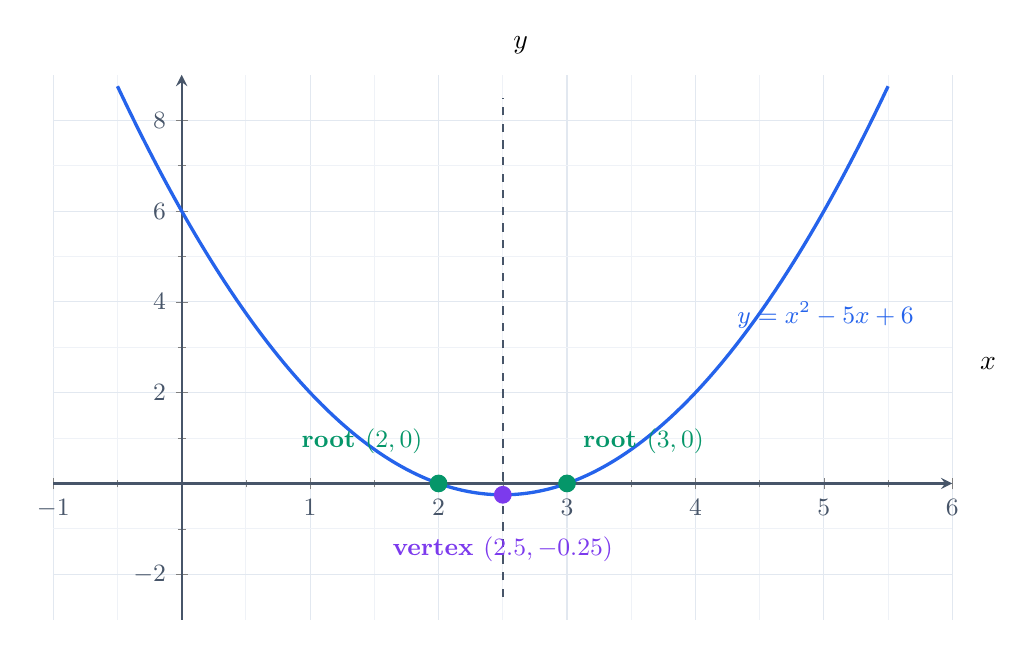
\begin{tikzpicture}
\begin{axis}[
  width=13cm,
  height=8.5cm,
  axis lines=middle,
  axis line style={axisgray, thick},
  xlabel={$x$},
  ylabel={$y$},
  xlabel style={at={(axis description cs:1.02,0.47)},anchor=west},
  ylabel style={at={(axis description cs:0.52,1.02)},anchor=south},
  xmin=-1,
  xmax=6,
  ymin=-3,
  ymax=9,
  xtick={-1,0,1,2,3,4,5,6},
  ytick={-2,0,2,4,6,8},
  grid=both,
  minor tick num=1,
  major grid style={gridgray},
  minor grid style={gridgray!55},
  tick label style={font=\small, text=axisgray},
  label style={font=\bfseries},
  samples=220,
  clip=false,
]
\addplot[curveblue, very thick, domain=-0.5:5.5] {x^2-5*x+6};
\addplot[rootgreen, only marks, mark=*, mark size=3pt] coordinates {(2,0) (3,0)};
\addplot[vertexviolet, only marks, mark=*, mark size=3pt] coordinates {(2.5,-0.25)};
\addplot[axisgray, dashed, thick, domain=-2.5:8.5] coordinates {(2.5,-2.5) (2.5,8.5)};
\node[font=\small\bfseries, text=rootgreen, anchor=south east] at (axis cs:1.95,0.45) {root $(2,0)$};
\node[font=\small\bfseries, text=rootgreen, anchor=south west] at (axis cs:3.05,0.45) {root $(3,0)$};
\node[font=\small\bfseries, text=vertexviolet, anchor=north] at (axis cs:2.5,-0.95) {vertex $(2.5,-0.25)$};
\node[font=\small\bfseries, text=curveblue, anchor=south west] at (axis cs:4.25,3.2) {$y=x^2-5x+6$};
\end{axis}
\end{tikzpicture}
\end{document}
